\documentclass{tufte-handout}

\usepackage[french]{babel}
\usepackage[utf8]{inputenc}
\usepackage[T1]{fontenc}
\usepackage{amsmath, amsthm, amsfonts}
\usepackage{siunitx}
\usepackage{tikz}
\usepackage{hyperref}
%\usepackage[backend=biber, autocite=footnote]{biblatex}
\usepackage{xcolor}
\usepackage{caption}
\usepackage{booktabs}
\usepackage{mathtools}

\tikzset{>=latex}
\usetikzlibrary{calc,decorations.pathreplacing}
\sisetup{locale=FR, per-mode=symbol}

\newcommand{\abs}[1]{\left| #1 \right|}
%\renewcommand{\vec}[1]{\ensuremath{\overrightarrow{\boldsymbol{\mathrm{ #1 }}}}}
\newcommand{\rhat}{\vec{\hat{r}}}
\newcommand{\xhat}{\vec{i}}
\newcommand{\yhat}{\vec{j}}
\newcommand{\zhat}{\vec{k}}
\newcommand{\real}{\mathbb{R}}
\newcommand{\der}[2]{\frac{\mathrm{d}#1}{\mathrm{d}#2}}
\newcommand{\pder}[2]{\frac{\partial #1}{\partial #2}}
\newcommand{\dif}{\mathrm{d}}
\newcommand{\ddif}{\,\mathrm{d}}
\newcommand{\grad}{\vec{\nabla}}
\newcommand{\exemple}[1]{\begin{fullwidth}#1\end{fullwidth}}
\newcommand{\norm}[1]{\lVert #1 \rVert}
\newcommand{\vu}{\vec{u}}
\newcommand{\vv}{\vec{v}}
\newcommand{\vr}{\vec{r}}
\newcommand{\va}{\vec{a}}
\newcommand{\vF}{\vec{F}}
\newcommand{\vecxyz}[3]{#1 \xhat + #2 \yhat + #3 \zhat}
\newcommand{\vecxy}[2]{#1 \xhat + #2 \yhat}

\theoremstyle{definition}
\newtheorem*{defn}{Definition}



\title{Exercices sur le mouvement des projectiles}
\date{}

\begin{document}

\maketitle
\vspace{0.5cm}

\section{Exercice I -- Basketball}

Une personne lance un ballon de basket-ball.  Au moment où celui-ci quitte
ses mains, il est à 2 m au-dessus du sol et voyage à \SI{7.5}{m/s} selon un
angle de \SI{55}{\degree} vers le haut par rapport à l'horizontale.  Le
ballon pénètre dans un panier dont l'anneau est à \SI{3.05}{m} au-dessus du
sol.  On désire calculer
\begin{marginfigure}
  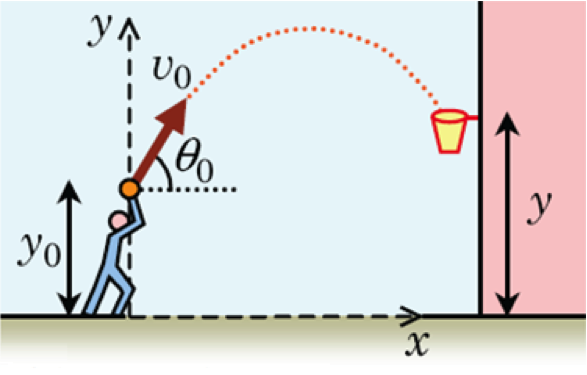
\includegraphics[scale=0.6]{basket.png}
\end{marginfigure}

\begin{enumerate}
  \item le temps de vol du ballon
  \item la hauteur maximale du ballon par rapport au sol
  \item l'angle que forme la trajectoire du ballon avec l'horizontale lorsqu'il
        pénètre dans le panier
\end{enumerate}


\paragraph{Solution}
Faisons d'abord un schéma pour représenter ce qui se passe.  La figure
ci-contre montre le lanceur du ballon, le panier, la trajectoire du ballon, un
système d'axes et les quantités données dans le problème.

Nous pouvons ensuite faire un inventaire de l'information que nous avons à
notre disposition.

\begin{itemize}
  \item vitesse initiale, $\vec{v}_0$: $v_0 = \SI{7.5}{m/s}$,
    $\theta_0 = \SI{55}{\degree}$;
  \item hauteur initiale, $y_0 = \SI{2}{\meter}$;
  \item hauteur finale, $y = \SI{3.05}{\meter}$;
  \item accélération gravitationnelle, $a_y =
    -g = \SI{-9.8}{\meter\per\second\squared}$.
\end{itemize}

\begin{enumerate}
  \item
    Le mouvement vertical est un MRUA avec une accélération vers le bas égale à
    l'accélération gravitationnelle terrestre.  Les composantes en $y$ de la
    position et de la vitesse sont donc
    \begin{align}
      y   &= y_0 + v_{0y}t + \frac{1}{2} a_y t^2 \label{eqn:basket1}\\
      v_y &= v_{0y} + a_y t \label{eqn:basket2}
    \end{align}
    On cherche le temps de vol du ballon.  Nous remarquons qu'avec la position
    finale du ballon, l'équation \ref{eqn:basket1} ne contient qu'une seule
    inconnue, soit le temps.  Nous pouvons donc résoudre directement à partir
    de cette équation.
    \begin{align*}
      y &= y_0 + v_{0y} t + \frac{1}{2} a_y t^2 \\
      0 &= \frac{1}{2} a_y t^2 + v_{0y} t + (y_0 - y) \\
      t &= \frac{-v_{0y} \pm \sqrt{v_{0y}^2 - 2a_y(y_0 - y)}}{a_y}
    \end{align*}
    La composante $y$ de la vitesse initiale est calculée en faisant un peu de
    trigonométrie:
    \begin{align*}
      v_{0y} &= v_0 \sin \theta_0
    \end{align*}
    En substituant dans l'équation précédente nous obtenons
    \begin{align*}
      t &= \frac{-v_{0}\sin\theta_0 \pm \sqrt{v_{0}^2\sin^2\theta_0 - 2a_y(y_0 - y)}}{a_y}
    \end{align*}
    La résolution numérique de l'équation donne deux solutions possibles soit
    \begin{align*}
      t_1 &= \SI{0.2041486}{\second} \\
      t_2 &= \SI{1.049656}{\second}
    \end{align*}
    La première valeur correspond au moment où le ballon est en ascension peu
    de temps après avoir quitté les mains du joueur.  Le temps recherché est
    donc le second.  Le ballon est resté dans les airs pendant un temps
    \[
      \boxed{t = \SI{1.05}{\second}}
    \]


  \item On cherche maintenant la hauteur maximale du ballon par rapport au sol.
    On sait qu'au point le plus haut de sa trajectoire, la vitesse verticale du
    ballon est nulle.  Par conséquent on peut utiliser l'équation
    \ref{eqn:basket2} pour déterminer le temps auquel le ballon atteint son
    point le plus haut, puis remplacer ce temps dans l'équation
    \ref{eqn:basket1} pour déterminer la hauteur à laquelle il se trouve.

    Si $t_m$ est le temps auquel la hauteur maximale est atteinte, alors la
    vitesse à ce moment est nulle
    \begin{align*}
      \SI{0}{\meter\per\second} &= v_{0y} + a_y t_m \\
      t_m &= \frac{-v_{0y}}{a_y} 
    \end{align*}
    On remplace dans l'équation \ref{eqn:basket1} pour obtenir la hauteur
    maximale $y_m$.
    \begin{align*}
      y_m &= y_0 + v_{0y} \frac{-v_{0y}}{a_y} + \frac{1}{2}
             a_y \left(\frac{-v_{0y}}{a_y}\right)^2 \\
          &= y_0 - \frac{v_{0y}^2}{2a_y} \\
    \end{align*}
    En remplaçant par les valeurs numériques nous obtenons
    \[
      \boxed{y_m = \SI{3.93}{\meter}}
    \]

  \item Pour trouver l'angle formé par la trajectoire du ballon avec
    l'horizontale, on n'a qu'à trouver l'angle entre le vecteur vitesse et
    l'horizontale au point où le ballon arrive au panier.

    \begin{marginfigure}
      \begin{tikzpicture}[scale=1]
        \fill (0, 0) circle (0.3);
        \draw[dashed] (-3, 2) parabola (0, 0);
        \draw[->, very thick] (0, 0) -- (-43.9:2) node[anchor=north west] {$\vec{v}$};
        \draw[dashed] (0, 0) -- (2, 0);
        \draw (0.6, 0) arc (0:-43.9:0.6);
        \node at (0.7, -0.3) {$\theta$};
      \end{tikzpicture}
    \end{marginfigure}

    Appelons l'angle entre l'axe des $x$ et la vitesse finale $\theta$.  On
    peut trouver cet angle si on connaît les deux composantes de la vitesse
    finale.  Comme il n'y a aucune accélération horizontale, la composante $x$
    de la vitesse finale est la même que celle de la vitesse initiale
    \[
      v_x = v_{0x}
    \]
    Pour trouver la composante $y$ de la vitesse finale, nous pouvons utiliser
    l'équation \ref{eqn:basket2} avec le temps trouvé au point 1.
    \begin{align*}
      v_y = v_{0y} + a_yt
    \end{align*}
    Enfin,
    \begin{align*}
      \tan \theta &= \abs{\frac{v_y}{v_x}} \\
      \theta &= \arctan\abs{\frac{v_y}{v_x}}
    \end{align*}
    \[
      \boxed{\theta = \SI{43.9}{\degree}}
    \]

\end{enumerate}

\newpage

\section{Exercice II -- Les pirates!}

Un bateau pirate est muni d'un canon dont le tube forme un angle de
\SI{30}{\degree} avec l'horizontale. Un boulet tiré par ce canon atteint un
autre bateau situé à \SI{171}{\meter} de distance.  On désire déterminer le
module de la vitesse initiale du boulet.

On suppose que les bateaux sont immobiles et que la cible est à la même
hauteur que la bouche du canon.

\paragraph{Solution}

Faisons d'abord un schéma pour représenter ce qui se passe.  La figure
ci-contre montre les deux bateaux, un système d'axes et les quantités données
dans le problème.

Nous pouvons ensuite faire un inventaire de l'information que nous avons à
notre disposition.

\begin{marginfigure}
  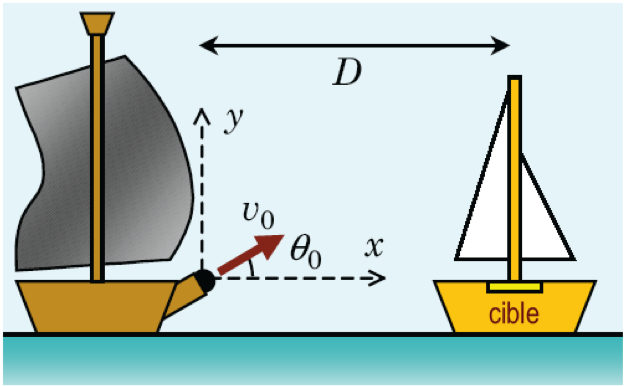
\includegraphics[scale=0.6]{pirates.png}
\end{marginfigure}

\begin{itemize}
  \item vitesse initiale, $\vec{v}_0$: $\theta_0 = \SI{30}{\degree}$;
  \item position initiale, $\vec{r}_0 = \vec{0}\si{\meter}$;
  \item hauteur finale, $y = \SI{0}{\meter}$;
  \item accélération gravitationnelle, $a_y =
    -g = \SI{-9.8}{\meter\per\second\squared}$;
  \item distance entre les bateaux, $D = \SI{171}{\meter}$.
\end{itemize}

Nous connaissons donc la position finale du boulet de canon :
\[
  \vec{r} = D\xhat + 0\yhat
\]

Le mouvement horizontal est un MRU parce qu'aucune accélération horizontale
n'est présente.  De plus, la composante $x$ de la position initiale est nulle.
Par conséquent les composantes en $x$ de la position et de la vitesse sont
données par les relations suivantes
\begin{align}
  x   &= v_{0x} t \label{eqn:piratex} \\
  v_x &= v_{0x} \label{eqn:piratevx}
\end{align}

La composante vertical du mouvement est un MRUA donc les équations du mouvement
sont
\begin{align}
  y   &= v_{0y} t + \frac{1}{2} a_y t^2 \label{eqn:piratey} \\
  v_y &= v_{0y} + a_y t \label{eqn:piratevy}
\end{align}

Si on évalue les équations \ref{eqn:piratex} et \ref{eqn:piratey} au moment où
le boulet touche la cible $t_c$, on obtient
\begin{align*}
  D &= v_{0x}t_c \\
  0 &= v_{0y} t_c + \frac{1}{2} a_y t_c^2 \\
\end{align*}
Nous pouvons aussi utiliser la trigonométrie pour exprimer les composantes de
la vitesse initiale en fonction du module et de l'angle.
\begin{align*}
  D &= v_{0}\cos\theta_0 t_c \\
  0 &= v_{0}\sin\theta_0 t_c + \frac{1}{2} a_y t_c^2 \\
\end{align*}
Isolons $t_c$ dans la première équation
\begin{align*}
  t_c = \frac{D}{v_0\cos\theta_0} 
\end{align*}
puis remplaçons dans la seconde équation divisée par $t_c$
\begin{align*}
  v_0 \sin\theta_0 + \frac{1}{2} a_y \frac{D}{v_0\cos\theta_0} &= 0 \\
  v_0 \sin\theta_0 &= -\frac{a_y D}{2v_0 \cos\theta_0} \\
  v_0^2 &= -\frac{a_y D}{2\cos\theta_0\sin\theta_0} \\
  v_0 &= \sqrt{-\frac{a_y D}{2\cos\theta_0\sin\theta_0}}
\end{align*}
\[
  \boxed{v_0 = \SI{44.0}{\meter\per\second}}
\]

\end{document}

